\documentclass[fleqn]{article}

\usepackage{polski}
\usepackage[utf8]{inputenc}
\usepackage[polish]{babel}
\usepackage{parskip}
\usepackage{icomma}
\usepackage[a4paper,includeheadfoot,margin=2.54cm]{geometry}
\usepackage{float}
\usepackage{graphicx}
\usepackage{amsmath}
\usepackage{subcaption}



\renewcommand\thesection{\arabic{section}.}
\renewcommand\thesubsection{\arabic{section}. \alph{subsection})}
\renewcommand\thesubsubsection{}

\brokenpenalty=1000
\clubpenalty=1000
\widowpenalty=1000

\title{TM -- Laboratorium 1.}
\author{Krystian Chachuła \\ Dawid Gruszczyński \\ Marcin Skrzypkowski}

\begin{document}

\maketitle

\setcounter{page}{0}
\thispagestyle{empty}

\pagebreak

\setcounter{page}{1}

\section{Pierwsze laboratorium}

Na pierwszym laboratorium mieliśmy za zadanie oswoić się z układem FPGA symulującym mikroprocesor Z80 przez rozpoznanie podstawowych instrukcji wejścia/wyjścia oraz pamięci. Ćwiczenie składało się z trzech punktów: przedstawienia podstawowych instrukcji na oscyloskopie, złożenia układu atywującego sygnał $\overline{WAIT}$ na zadaną ilość taktów po spełnieniu określonych warunków oraz zbudowania układu pułakpującego procesor w tym sygnale do czasu wyzwolenia przełącznikiem bistabilnym. 

\section{Odczytywanie przebiegów instrukcji na oscyloskopie}
Pierwsze zadanie polegało na obserwacji i opisie pięciu przebiegów sygnałów procesora: wczytywanie i zapisywanie do pamięci, wczytywanie i zapisywanie do przestrzeni wejścia/wyjśćia oraz cykl pobierania i dekodowania kodu instrukcji.
W celu realizacji zadania napisaliśmy prosty program w Assembly Z80, który po uruchomieniu w aplikacji NoICE i włączeniu trybu RUN pozwalał na obserwację wyżej wymienionych przebiegów.

%TODO: wstawić kod do zadania 1
`
Cykl fetch:
Na początku realizacji każdego polecenia mikroprocesor pobiera kod instrukcji, co jest sygnalizowane stanem niskim na wyjściach $\overline{MREQ}$, $\overline{RD}$ oraz $\overline{M1}$. Następnie następuje odświeżenie pamięci sygnalizowane stanem niskim jedynie na wyjściu $\overline{MREQ}$ (oraz $\overline{RFSH}$, lecz nie widć tego na oscylogramie). W trakcie odświeżania dekodowany jest także kod pobranej instrukcji.
Powyższą instrukcję można zaobserwować w bloku nr1 na poniższym zdjęciu

Cykl odczytu z pamięci
Podczas tego cyklu zaznaczonego w bloku nr2 nastęuje pobranie argumentów do wykonania polecenia OUT, a więc odczyt z pamięci.
Sygnalizowane jest to niskim stanem na wyjściach $\overline{MREQ}$ i $\overline{RD}$
%TODO: sprawwdzić jakie polecenie

Zapis do układów wejścia/wyjścia:
Podczas cyklu zaznaczonego w bloku nr 3 następuje zapis do układów wejścia/wyjścia realizowany przez instrukcję OUT, sygnalizowane jest to stanem niskim na wyjściach $\overline{IORQ}$ i $\overline{WR}$ ($\overline{WR}$ nie jest widoczne na oscylogramie).
%TODO do sprawdzenia

Odczyt z przestrzeni wejścia/wyjścia:
Podczas cyklu zaznaczonego w bloku nr 4 następuje udczyt z układów wejścia/wyjścia realizowany przez instrukcję IN, sygnalizowane jest to stanem niskim na wyjściach $\overline{IORQ}$ i $\overline{RD}$.
%TODO sprawdzić

Cykl zapisu do pamięci:
Podczas cyklu zaznaczonego w bloku nr 5 następuje zapis do pamięci realizowany przez isntrukcję LD, sygnalizowane jest to stanem niskim na wyjściach $\overline{MREQ}$ i $\overline{WR}$ ($\overline{WR}$ nie jest widoczne na oscylogramie).
   




\begin{figure}[H]
	\centering
	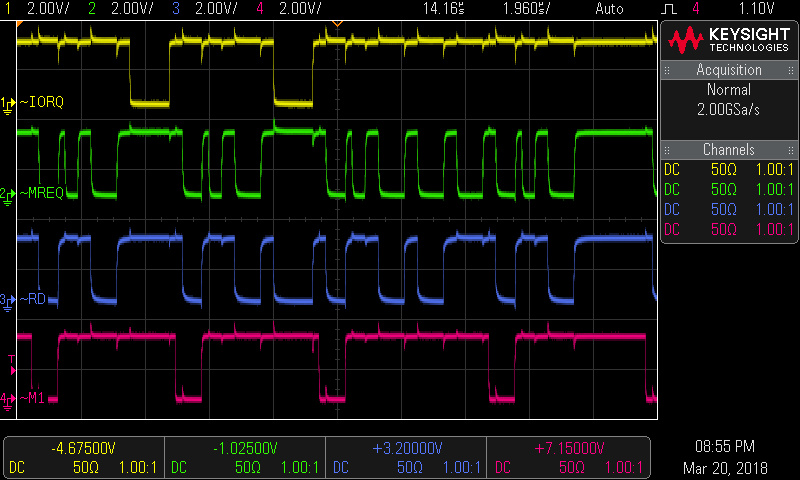
\includegraphics[width=0.75\textwidth]{img/1a.png}
	\caption{}
\end{figure}

\section{Generowanie sygnału opóźniającego}

Naszym zdaniem było wstawianie dwóch taktów opóźnienia przy odczytywaniu danych z przestrzeni wejścia/wyjścia. Procesor autoamatycznie wstawia jeden takt opóźniena przy przy wykonywaniu instrukcji dotyczących tej przestrzeni, zatem łącznie mieliśmy uzyskać trzy takty opóźniena.

Pierwszą naszą czynnościa było stworzenie funkcji logicznej, która przymowała wartość $1$, gdy był spełniony warunek z treści zadania lub $0$ w pozostałych przypadkach. Następnie zaprojektowaliśmy układ kombinacyjny realizujący tę funkcję. Początkowo wykorzystaliśmy bramki \textit{NAND} oraz \textit{NOT}, ale ze względu na trudność modyfikacji oraz małą przejrzystość takiego układu finalnie zdecydowaliśmy, że użyjemy multipleksera.

% TODO: napisać o module SML-3 z rejestrem
Do odliczania taktów zegara procesora zdecydowaliśmy się użyć rejestru przesuwnego z modułu SML-3. Pozwala on zliczyć maksymalnie 4 takty zegara, więc biorąc pod uwagę wbudowany takt oczekiwania byliśmy w stanie dodać maksymalnie 3 takty. ale było to wystarczające do wykonania zadania. Wejściem zegarowym rejestru był zanegowany sygnał zegarowy,ponieważ sygnał WAIT był próbkowany przez procesor podczas opadającego zbocza zegara, więc każde przesunięcie zawartości rejestru oznaczało wydłużenie sygnału opóźniającego o jeden takt.  Alternatywą do naszego rozwiązania było użycie licznika, lecz rejestr był rozwiązaniem prostszym.

Ładowanie rejestru oraz przesuwanie odbywało się przez podłączenie do wejścia \textit{s0} sygnału $\overline{IORQ}$: w stanie wysokim następowało ładowanie rejestru, a w stanie niskim przesuwanie.

Ilość wymaganych przez zadanie taktów zegara była ładowana do rejestru z modułu przełączników szesnastkowych IN\_4xHEX.

Wyjście multipleksera oraz najmniej znaczący bit rejestru zostały doprowadzone do wejść bramki \textit{NAND}. W ten sposób otrzymaliśmy wymagany sygnał $\overline{WAIT}$.

%TODO: wstawić kod do zadania 2

\begin{figure}[H]
	\centering


%	\subfloat[blabla]{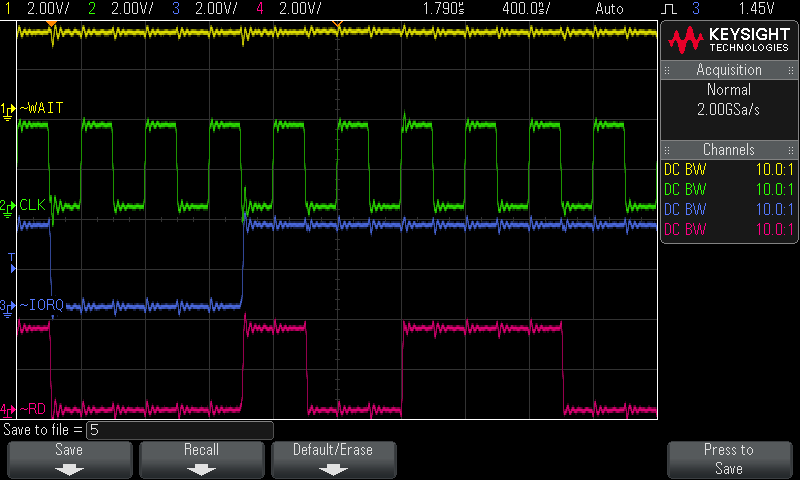
\includegraphics[width=2.5in]{img/2a.png}}
%	\subfloat[blabla]{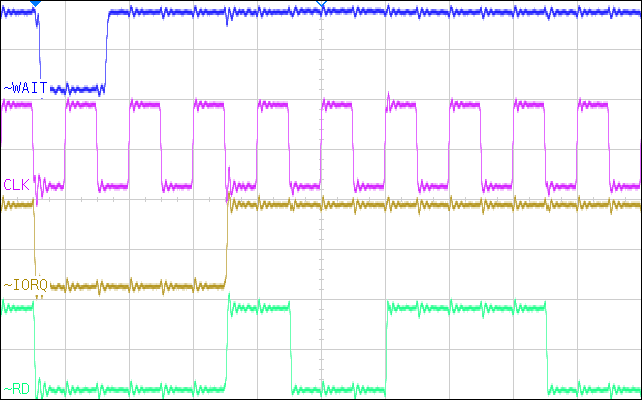
\includegraphics[width=2.5in]{img/2b.png}}	

	\begin{subfigure}[b]{0.49\textwidth}
		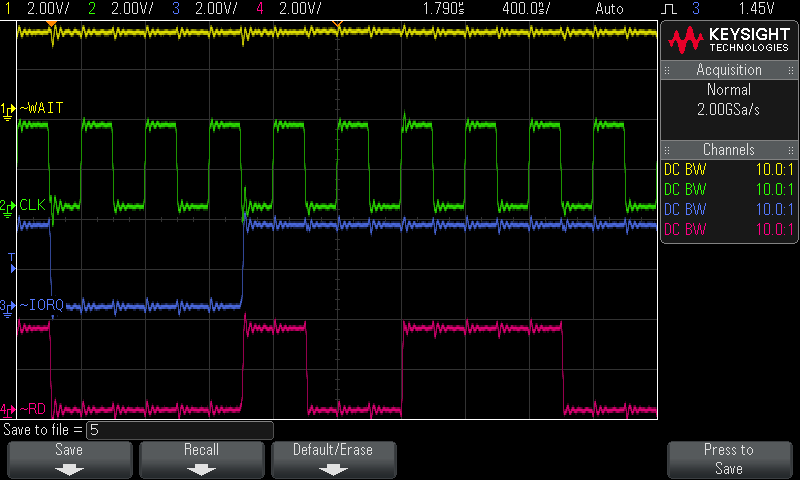
\includegraphics[width=\textwidth]{img/2a.png}
		\caption{}
	\end{subfigure}
	\begin{subfigure}[b]{0.49\textwidth}
		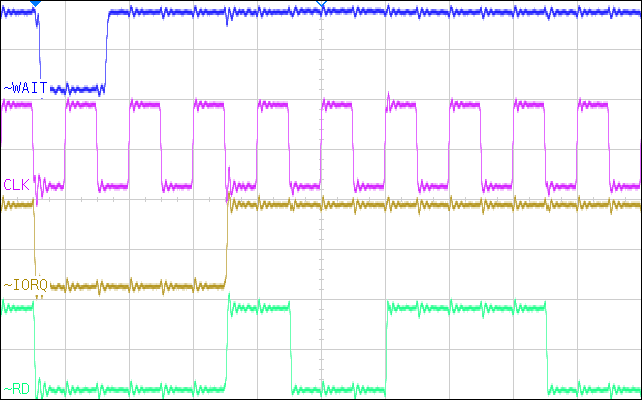
\includegraphics[width=\textwidth]{img/2b.png}
		\caption{}
	\end{subfigure}
	\begin{subfigure}[b]{0.49\textwidth}
		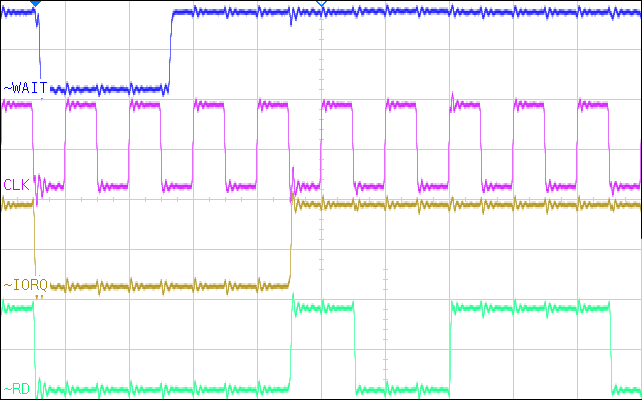
\includegraphics[width=\textwidth]{img/2c.png}
		\caption{}
	\end{subfigure}
	\begin{subfigure}[b]{0.49\textwidth}
		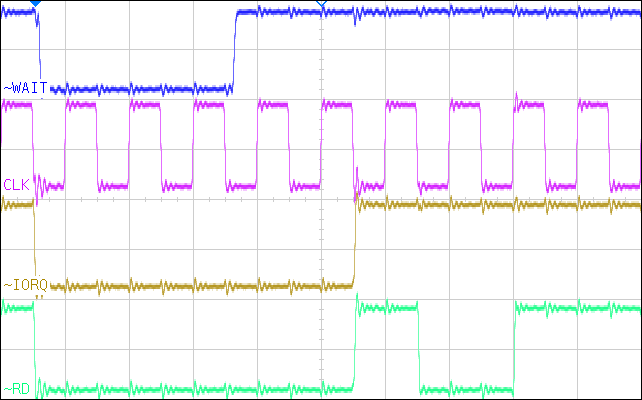
\includegraphics[width=\textwidth]{img/2d.png}
		\caption{}
	\end{subfigure}
	\begin{subfigure}[b]{0.49\textwidth}
		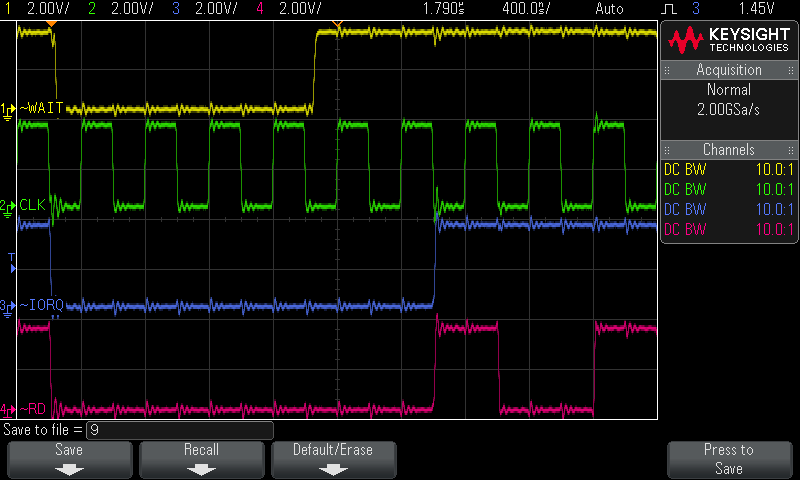
\includegraphics[width=\textwidth]{img/2e.png}
		\caption{}
	\end{subfigure}
	\caption{}
\end{figure}

\section{Wstrzymywanie pracy procesora}

Ostatnim zadaniem była modyfikacja poprzedniego układu w taki sposób, aby zamiast wstawiać takty oczekiwania, generować sygnał $\overline{WAIT}$ do momentu uzyskania zbocza przełącznika.
Zdecydowaliśmy się zastąpić rejestr przerzutnikiem typu D, gdyż element zliczający nie był już potrzebny, a wystarczył prosty układ z pamięcią. Przerzutnik pozwalał nam też na trywialne wykrywanie zbocza przełączania przez podłączenie go do wejścia zegarowego.
W normalnych warunkach (gdy procesor nie wpadał w pułapkę) przerzutnik był zerowany seygnałem \textit{M1}. Do wejścia D była podpięty sały sygnał wysoki, dzięki czemu zbocze przełącznika powodowało dezaktywację sygnału $\overline{WAIT}$ poprzez resetowanie wyjścia $\overline{Q}$ przerzutnika.

Układ multipleksera pozostawiliśmy bez zmian, natomiast do bramki NAND, z której wychodzi sygnał $\overline{WAIT}$, zamiast najmniej znaczącego bitu rejestru podłączyliśmt wyjście $\overline{Q}$ przerzutnika.

%TODO: wstawić kod z zadania 3

\begin{figure}[H]
	\centering
	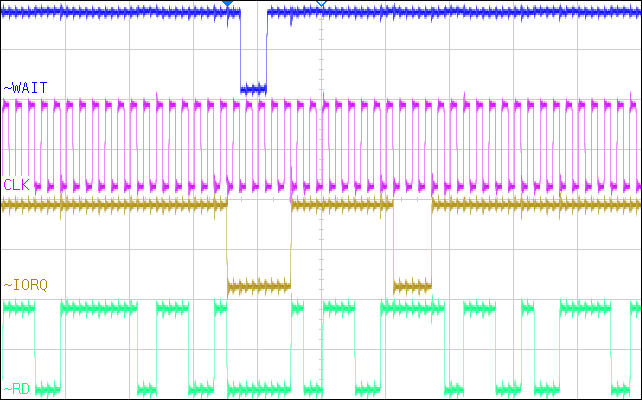
\includegraphics[width=0.75\textwidth]{img/3a.png}
	\caption{}
\end{figure}

\begin{figure}[H]
	\centering
	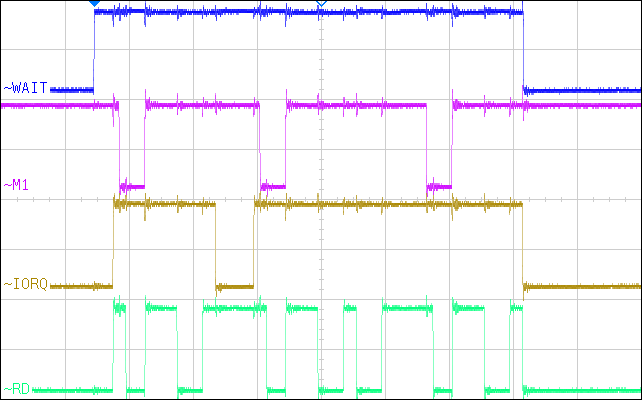
\includegraphics[width=0.75\textwidth]{img/3b.png}
	\caption{}
\end{figure}

\begin{figure}[H]
	\centering
	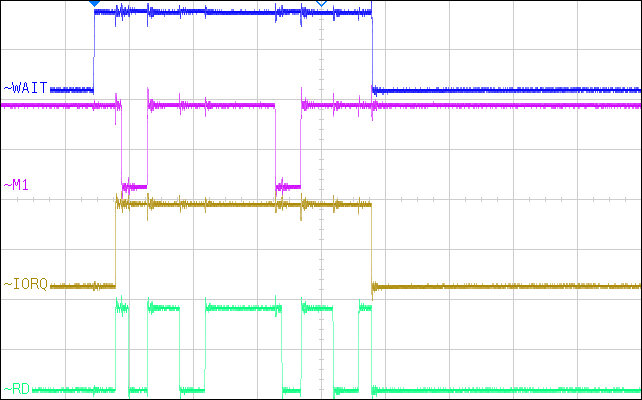
\includegraphics[width=0.75\textwidth]{img/3c.png}
	\caption{}
\end{figure}

\section{Problemy}

Podczas prób budowy zaprojektowanych układów natrafiliśmy na kilka problemów, które ostatecznie udało nam się rozwiązać.
Jednym z nich były szybko zanikające sygnały. Było to spowodowane podłączeniem dwóch modułów BNC. Pomimo uzyskania prawidłowego działania układu sygnał $\overline{WAIT}$ był zbyt słaby, aby procesor mógł zauważyć jego zmiany- przez cały czas traktował jego stan jako niski. Aby uniknąć tej sytuacji podczas testowania układu korzystaliśmy z sond dołączonych do oscyloskopu.
Kolejnym problemem było podłączenie licznika do układu z zadania drugiego. Podczas testów okazało się, że sygnał przeniesienia znikał zbyt szybko, więc procesor nie zauważał zmiany sygnału $\overline{WAIT}$ i nie mógł zmienić stanu wyjść, wobec teego licznik zaczynal liczyć od zera. Powodowało to zarzymanie procesora. Problem następował przy zliczaniu do 16. Znaleźliśmy dwa rozwiązania tego problemu, jednym było zliczanie do 8 i wykorzystanie najstarszego bitu jako bit przeniesienia lub użycie rejestru. Ostatecznie zdecydowaliśmy się na wykorzystanie drugiej opcji.


\end{document}
